\section{Firewall e NAT}
\subsection{Firewall}
Un firewall è un meccanismo di protezione che un host della rete può implementare.
Ci sono varie tipologie di firewall ma tutti quanti sono pensati per vietare determinati accessi e permetterne altri.
Possiamo ad esempio consentire ad una macchina di accedere ad alcuni host tranne ad altri, bloccare tutto il traffico http in uscita da una rete, permettere solo il traffico smtp, ecc, ecc.

\subsubsection{Perché?}
Le reti ed i computer connessi ad Internet vanno protetti da accessi indesiderati ed eventualmente malware.

\subsubsection{Come?}
Può essere un sistema hardware o software che monitora le connessioni in ingresso ed in uscita e su questi pacchetti applica delle regole.
Possiamo avere:
\begin{itemize}
    \item firewall al network layer: si tratta di packet filtering, permettono di interpretare pacchetti a livello TCP/IP quindi analizzano header IP, TCP ed UDP
    
    \item firewall al livello applicazione: si tratta di deep packet inspection, oltre a comprendere i segmenti IP, TCP ed UDP possono comprendere anche dati a livello applicazione.
    Possiamo quindi avere più consapevolezza del contesto dei messaggi.
\end{itemize}

\subsubsection{Packet filtering}
Possiamo usare due tecniche:
\begin{itemize}
    \item stateless: ogni pacchetto viene analizzato in base a campi statici come indirizzo di sorgente o destinazione
    
    \item stateful: tiene traccia delle connessioni TCP e degli scambi UDP in corso e discrimina le connessioni legittime da quelle sospette.
    Ha un minimo di contesto in più rispetto all' approccio stateless.
\end{itemize}

\subsubsection{Tabelle di regole}
Il firewall contiene una tabella di regole, ogni riga di questa tabella è quindi una regola composta da:
\begin{itemize}
    \item \emph{criteria}: caratteristiche del pacchetto
    \item \emph{target}: azione da intraprendere al match tra DROP e ACCEPT
\end{itemize}
Es:
\begin{table}[ht!]
    \centering
    \begin{tabular}{c|c|c|c|c|c}
        Indice & IP sorgente & \thead{Porta \\ sorgente} & IP destinatario & \thead{Porta \\ dest} & Azione  \\
        \hline
        1 & 131.114.0.0/16 & & 131.114.54.4 & 80 & DROP \\
        2 & 0.0.0.0 & 23 & 112.143.2.2 &  & ACCEPT \\
    \end{tabular}
\end{table}
La prima riga indica che i pacchetti provenienti da IP nella rete 131.114.0.0/16 da qualsiasi porta sorgente e che sono diretti all' host con IP 131.114.54.4 verso la porta 80 devono venire scartati.

Il firewall quindi scorre le regole dall' alto verso il basso e quando trova una riga che matcha i dati del pacchetto che si sta considerando esegue l' azione specificata.

Per ogni pacchetto viene eseguita una sola regola in quanto appena una matcha si esegue l' azione specificata e si va al prossimo pacchetto.

\subsubsection{Regola di default}
Se nessuna regola nella tabella matcha il pacchetto si hanno delle regole di default in base al firewall:
\begin{itemize}
    \item firewall inclusivo: se l' azione di default è di droppare il pacchetto.
    Più sicuro ma più scomodo.
    \item firewall esclusivo: se l' azione di default è quella di accettare il pacchetto
\end{itemize}

\subsubsection{Esempio}
Data la rete locale 222.22.0.0/16 vogliamo far si che:
\begin{itemize}
    \item sia impedito l' accesso a Internet dall' interno della rete
    \item sia consentito alla rete esterna 111.11.0.0/16 di accedere alla sottorete locale 222.22.22.0/24
    \item sia impedito alla sottorete esterna 111.11.11.0/24 di accedere alla sottorete locale 222.22.22.0/24
\end{itemize}
\begin{table}[ht!]
    \centering
    \begin{tabular}{c|c|c|c|c|c}
        Indice & IP sorgente & \thead{Porta \\ sorgente} & IP destinatario & \thead{Porta \\ dest} & Azione  \\
        \hline
        1 & 111.11.11.0/24 & & 222.22.22.0/24 & & DROP \\
        2 & 111.11.0.0/16 & & 222.22.22.0/24 & & ACCEPT \\
        3 & 0.0.0.0 & & 0.0.0.0 & & DROP \\
    \end{tabular}
\end{table}

\subsection{netfilter e iptables}
\subsubsection{netfilter}
E' la componete del kernel linux che offre le funzionalità di:
\begin{itemize}
    \item statelss/stateful packet filtering
    \item NA[P]T
    \item packet mangling (manipolazione generica)
\end{itemize}

\subsubsection{iptables}
E' il programma da linea di comando per configurare le tabelle di regole da far applicare a netfilter.

Lavora su diverse tabelle (table), ognuna è dedicata ad una funzionalità.
Noi vedremo:
\begin{itemize}
    \item \verb{filter{: è la tabella di filtraggio dei pacchetti
    \item \verb{nat{: è la tabella che si occupa di gestire del network address translation
\end{itemize}

Ogni tabella contiene diverse catene (chain), ogni catena contiene una lista di regole da applicare ad una determinata categoria di pacchetti:
\begin{itemize}
    \item pacchetti in ingresso: pacchetti il cui destinatario siamo noi.
    La chain è la \verb{INPUT{

    \item pacchetti in uscita: pacchetti il cui mittente siamo noi.
    La chain è la \verb{OUTPUT{

    \item pacchetti in transito: pacchetti che dobbiamo instradare.
    Utilissimo quando usiamo una macchina Linux come firewall.
    La chain è la \verb{FORWARD{
\end{itemize}

\begin{figure}[H]
    \centering
    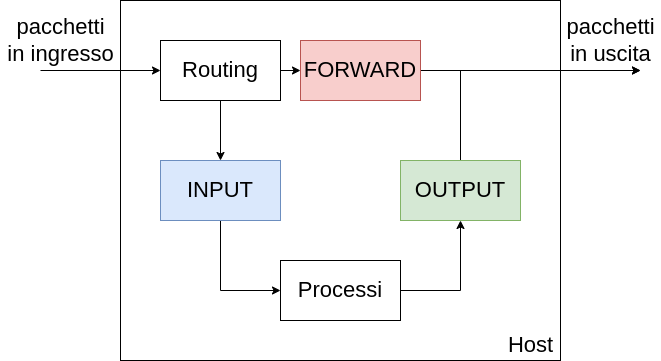
\includegraphics[width=250px]{images/4.1_Firewall/filter_chain.png}
\end{figure}

\subsubsection{Vedere le regole}
Per visualizzare le regole:
\begin{verbatim}
    iptables [-t table] -L [chain]
\end{verbatim}
se la tabella non è specificata viene selezionata in automatico \verb{filter{, se la catena non è specificata allora vengono elencate tutte le catene.

Es:
\begin{verbatim}
    iptables -L INPUT
\end{verbatim}
per vedere le regole della chain INPUT nella tabella \verb{filter{.
\begin{verbatim}
    iptables -t nat -L
\end{verbatim}
per vedere le regole di tutte le chain nella tabella \verb{nat{.


\subsubsection{Aggiunta di regole}
\begin{verbatim}
    iptables [-t table] -A chain <rule-specification>
\end{verbatim}
anche qui se non specifichiamo la tabella si usa la \verb{filter{ di default.
Per specificare una regola in una posizione specifica:
\begin{verbatim}
    iptables [-t table] -I chain [num] <rule-specification>
\end{verbatim}
se non si specifica l' indice la regola viene inserita in testa alla chain.


\subsubsection{Rimozione di regole}
\begin{verbatim}
    iptables [-t table] -D chain <rule-specification>
\end{verbatim}
oppure per indice:
\begin{verbatim}
    iptables -t table -D chain num
\end{verbatim}
Per rimuovere tutte le regole da una o più catene (flush):
\begin{verbatim}
    iptables [-t table] -F [chain]
\end{verbatim}
NB: anche cancellando tutto rimane la regola di default!

\subsubsection{Specificare la policy del firewall}
Per cambiare la regola di default (detta policy):
\begin{verbatim}
    iptables [-t table] -P target
\end{verbatim}

\subsubsection{Formato delle regole}
\emph{rule specification} è una stringa dove specificare:
\begin{itemize}
    \item \verb{-p{: protocollo (TCP, UDP, ICMP, ..)
    \item \verb{-s{: indirizzo IP sorgente
    \item \verb{-d{: indirizzo IP destinatario
    \item \verb{--sport{: porta sorgente
    \item \verb{--dport{: porta destinazione
    \item \verb{-i{: interfaccia di ingresso
    \item \verb{-o{: interfaccia di uscita
    \item \verb{-j{: azione (DROP/ACCEPT)
\end{itemize}


Es:
\begin{verbatim}
    iptables -A OUTPUT -p tcp -d 10.0.5.4 --dport 80 -j DROP
\end{verbatim}
Aggiungi la regola sulla chain di OUTPUT della tabella filter e specifica di droppare i pacchetti TCP con destinazione 10.0.5.4 verso la porta 80.


\begin{verbatim}
    iptables -A INPUT -p udp -s 121.0.0.0/16 -j ACCEPT
\end{verbatim}
Aggiungi la regola sulla chain di INPUT della tabella filter e specifica di accettare i pacchetti UDP che vengono dalla rete 121.0.0.0/16.


\begin{verbatim}
    iptables -A INPUT -p icmp -i eth0 -j DROP
\end{verbatim}
Aggiungi la regola sulla chain di INPUT della tabella filter e specifica di droppare i pacchetti icmp che vengono dalla interfaccia eth0.


\subsubsection{Salvataggio delle regole}
Le regole non vengono salvate, è quindi necessario reimpostarle all' avvio!
Per salvere le regole su file:
\begin{verbatim}
    iptables-save > file
\end{verbatim}
Per ricaricarle da file:
\begin{verbatim}
    iptables-restore < file
\end{verbatim}


\subsection{NAT e PAT}
Gli indirizzi IP sono scarsi, ad esempio un ISP potrebbe avere a disposizione una rete /16 con quindi solo 65534 hosts.
Se il numero di host supera questo valore potrebbe essere un problema.

Per parzialmente risolvere questo problema è stato inventato il NAT/PAT:
il router di confine casalingo ha un solo IP associato dall' ISP, all' interno della rete gli host hanno un certo indirizzamento detto privato, quando vogliono andare fuori il router di confine esegue una traduzione degli indirizzi.
All' atto pratico il traffico proveniente dall' interno della rete compare all' esterno come proveniente dal router stesso.

\begin{figure}[H]
    \centering
    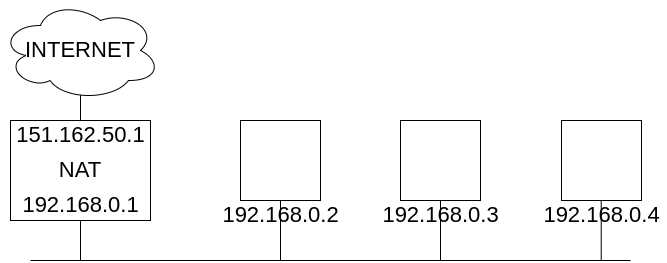
\includegraphics[width=200px]{images/4.1_Firewall/NAT.png}
\end{figure}
Verso l' interno la rete è 192.168.0.0/24, all' esterno invece il router ha ip 151.162.50.1.
Quando un host interno vuole trasmettere fuori, il router deve cambiare gli indirizzi IP dei pacchetti in un unico indirizzo IP, il suo!
Esempio:
\begin{itemize}
    \item l' host 192.168.0.2 vuole contattere 158.55.20.30
    \item invia il pacchetto al router
    \item il router modifica l' IP sorgente 192.168.0.2 con l' ip del router cioè 151.162.50.1 ed instrada il pacchetto
\end{itemize}
Al ritorno invece:
\begin{itemize}
    \item il router si vede arrivare un pacchetto con IP destinatario 151.162.50.1
    \item ne modifica l' IP destinatario in 192.168.0.2 ed instrada il pacchetto verso l' interno della rete
\end{itemize}

\subsubsection{PAT}
Se nella rete interna ci sono più host questo meccanismo non si può più fare con la sola traduzione dell' indirizzo IP.
Dobbiamo mappare più host della LAN in un solo IP pubblico, agiamo quindi sulle porte oltre che sull' IP: un pacchetto entrante avente una porta di destinazione (detta porta esterna) è tradotto in un pacchetto avente una porta differente (la porta interna).
NB: le porte non caratterizzano un processo in questo caso ma un solo host!
In pratica il numero di porta prende il posto dell' IP.

Questo meccanismo viene chiamato \emph{port address translation} - PAT.

\begin{figure}[H]
    \centering
    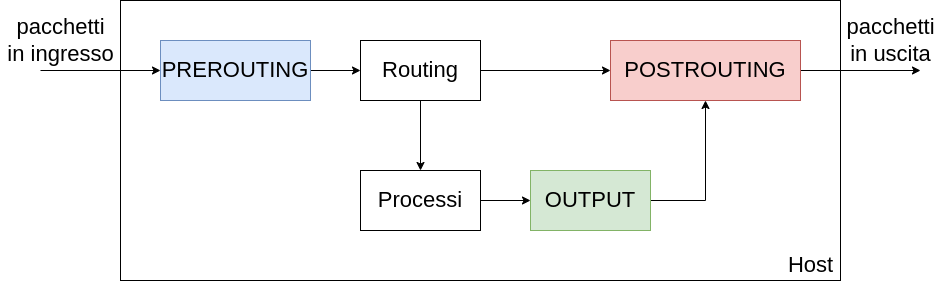
\includegraphics[width=330px]{images/4.1_Firewall/NAT_table.png}
\end{figure}

\subsubsection{iptables e NAT}
\verb{iptables{ gestisce il NA[P]T nella tabella \verb{nat{.
Abbiamo 3 catene:
\begin{itemize}
    \item \verb{PREROUTING{: fa destination NAT (D-NAT) cioè altera indirizzo/porta di destinazione dei pacchetti in arrivo
    \item \verb{OUTPUT{: fa destination NAT (D-NAT) dei pacchetti in uscita dai processi locali, prima del routing
    \item \verb{POSTROUTING{: fa source NAT (S-NAT) cioè altera indirizzo/porta sorgente dei pacchetti in uscita
\end{itemize}

Esempio: client 192.168.0.2 che vuole contattare 158.55.20.30 ma deve passare per il router 192.168.50.2, dobbiamo quindi tradurre l' indirizzo sorgente:
\begin{verbatim}
# iptables -t nat -A POSTROUTING -s 192.168.0.2 -j SNAT
    --to-source 151.162.50.2
\end{verbatim}
se vogliamo eseguire la traduzione per più host in modo da permettere il NAT di una intera rete:
\begin{verbatim}
# iptables -t nat -A POSTROUTING -s 192.168.0.0/24 -j SNAT
    --to-source 151.162.50.2:4001-4100
\end{verbatim}
traduce i pacchetti in ingresso dalla rete 192.168.0.0/24 sull' indirizo 151.162.50.2 assegnando una porta nel range 4001-4100.
Questo è necessario farlo in quanto nella stessa rete potremmo avere due host con porte sorgenti uguali, bisogna disambiguare.

Per tradurre indirizzi di destinazione (quindi quando la destinazione è nella nostra rete):
\begin{verbatim}
# iptables -t nat -A POSTROUTING -d 151.162.50.1 -j DNAT
    --to 192.168.0.2
\end{verbatim}
NB: non si specificano le porte quindi la traduzione viene eseguita per tutte le porte.

Se invece abbiamo più client nella stessa rete:
\begin{verbatim}
# iptables -t nat -A PREROUTING -p tcp --dport 80
    -j DNAT --to 19.168.0.55:80
\end{verbatim}
Per tutti i pacchetti in ingresso e diretti alla porta 80 TCP si deve eseguire D-NAT impostando l'IP 192.168.0.55 e la porta interna a 80.

\subsection{Catene filter e nat}
\begin{figure}[H]
    \centering
    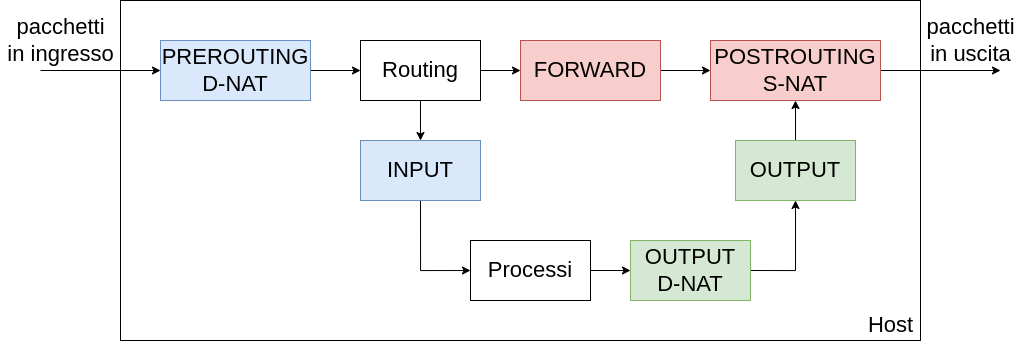
\includegraphics[width=330px]{images/4.1_Firewall/filter_nat_chains.png}
\end{figure}
Si noti che le catene filter e nat sono disposte in modo che quelle di filter vedano gli indirizzi e porte reali.
